\documentclass[sigplan,screen,nonacm]{acmart}

\usepackage{amsmath}
\usepackage{array}
\usepackage{booktabs}
\usepackage{etoolbox}
\usepackage{listings}
\usepackage{ragged2e}
\usepackage{tabularx}
\usepackage{tikz}
\usepackage{xcolor}
\usepackage{xurl}
\usetikzlibrary{arrows.meta,calc,decorations.pathreplacing,fit,matrix,positioning}

\settopmatter{printfolios=true, printccs=false, printacmref=false}

\newcommand{\einlang}{\textsc{Einlang}}
\newcolumntype{L}[1]{>{\RaggedRight\arraybackslash}p{#1}}
\newcolumntype{Y}{>{\RaggedRight\arraybackslash}X}
\emergencystretch=2em

\title[Einlang]{Einlang: Unifying Multidimensional Tensor Indexing, Declarative Recurrence, and Local Derivatives}
\author{Bowen Fu}
\renewcommand{\shortauthors}{Fu}

\definecolor{einKeyword}{RGB}{0,74,128}
\definecolor{einComment}{RGB}{90,104,120}
\definecolor{einString}{RGB}{153,79,0}
\definecolor{einFrame}{RGB}{188,194,201}
\definecolor{einBg}{RGB}{249,250,251}
\definecolor{figInk}{RGB}{29,44,61}
\definecolor{figLine}{RGB}{122,136,150}
\definecolor{figBlue}{RGB}{39,92,138}
\definecolor{figBlueBg}{RGB}{235,244,250}
\definecolor{figGreen}{RGB}{55,111,92}
\definecolor{figGreenBg}{RGB}{233,244,239}
\definecolor{figGold}{RGB}{167,116,39}
\definecolor{figGoldBg}{RGB}{250,244,230}
\definecolor{figRose}{RGB}{155,83,71}
\definecolor{figRoseBg}{RGB}{248,238,234}
\definecolor{figSlateBg}{RGB}{243,246,248}

\lstdefinelanguage{Einlang}{
  morekeywords={let,fn,if,else,match,use,where,sum,in,assert,print,true,false,as},
  sensitive=true,
  morecomment=[l]{//},
  morestring=[b]"
}

\lstdefinestyle{einlang}{
  language=Einlang,
  basicstyle=\ttfamily\footnotesize,
  keywordstyle=\color{einKeyword}\bfseries,
  commentstyle=\color{einComment}\itshape,
  stringstyle=\color{einString},
  breaklines=true,
  breakatwhitespace=true,
  columns=fullflexible,
  keepspaces=true,
  frame=single,
  framerule=0.4pt,
  rulecolor=\color{einFrame},
  backgroundcolor=\color{einBg},
  framesep=4pt,
  showstringspaces=false,
  aboveskip=0.4\baselineskip,
  belowskip=0.4\baselineskip
}

\lstdefinestyle{einlangwide}{
  language=Einlang,
  basicstyle=\ttfamily\small,
  keywordstyle=\color{einKeyword}\bfseries,
  commentstyle=\color{einComment}\itshape,
  stringstyle=\color{einString},
  breaklines=false,
  columns=fullflexible,
  keepspaces=true,
  frame=single,
  framerule=0.4pt,
  rulecolor=\color{einFrame},
  backgroundcolor=\color{einBg},
  framesep=5pt,
  showstringspaces=false,
  aboveskip=0.35\baselineskip,
  belowskip=0.35\baselineskip
}

\lstdefinestyle{pythoncode}{
  language=Python,
  basicstyle=\ttfamily\footnotesize,
  keywordstyle=\color{einKeyword}\bfseries,
  commentstyle=\color{einComment}\itshape,
  stringstyle=\color{einString},
  breaklines=true,
  breakatwhitespace=true,
  columns=fullflexible,
  keepspaces=true,
  frame=single,
  framerule=0.4pt,
  rulecolor=\color{einFrame},
  backgroundcolor=\color{einBg},
  framesep=4pt,
  showstringspaces=false,
  aboveskip=0.4\baselineskip,
  belowskip=0.4\baselineskip
}

\BeforeBeginEnvironment{lstlisting}{\par\noindent\begin{minipage}{\linewidth}}
\AfterEndEnvironment{lstlisting}{\end{minipage}\par}

\begin{document}

\begin{abstract}
Tensor programs need a source boundary that users can write directly and compilers can inspect. A common pattern still crosses several boundaries today: multidimensional indexing, recurrent state updates, and sensitivity queries are usually expressed through separate interfaces such as \texttt{einsum}-like functions, host-language loops or scan combinators, and \texttt{grad}/\texttt{backward} APIs. This fragmentation makes programs executable, but it hides the source facts that connect the mathematical definition to compiler analysis.

We present \einlang{}, a tensor language that integrates multidimensional indexed definitions, declarative recurrences, and local derivative requests in one binding environment. In \einlang{}, a recurrence is a named binding over an index space that declares its dependencies; later expressions can read points of that recurrence, and derivative requests can target either final results or intermediate bindings. The contribution is an executable abstraction boundary: indexed clauses define axes and covered domains, recurrent bindings define dependency graphs, and derivative requests denote shaped derivative values. A compiler can use these contracts to derive evaluation order and infer storage windows from static index offsets.

We ground the design in a working NumPy-backed implementation and examples that mix all three features, including recurrent sensitivity computations, storage-decision checks, and model-scale feasibility cases. The result is a source form for tensor programs that stays close to the mathematical description while preserving structure for compiler passes.
\end{abstract}

\begin{CCSXML}
<ccs2012>
<concept>
<concept_id>10011007.10011006.10011008</concept_id>
<concept_desc>Software and its engineering~General programming languages</concept_desc>
<concept_significance>500</concept_significance>
</concept>
<concept>
<concept_id>10011007.10011006.10011041</concept_id>
<concept_desc>Software and its engineering~Compilers</concept_desc>
<concept_significance>300</concept_significance>
</concept>
<concept>
<concept_id>10010147.10010257.10010282.10010292</concept_id>
<concept_desc>Computing methodologies~Automatic differentiation</concept_desc>
<concept_significance>300</concept_significance>
</concept>
</ccs2012>
\end{CCSXML}

\ccsdesc[500]{Software and its engineering~General programming languages}
\ccsdesc[300]{Software and its engineering~Compilers}
\ccsdesc[300]{Computing methodologies~Automatic differentiation}

\keywords{tensor languages, recurrence, indexing, automatic differentiation, storage analysis}

\maketitle

\section{Introduction}

\subsection{Motivation}

We design programs by building layers of abstraction. In tensor computing, three abstractions appear again and again: indexed contraction, which says which axes survive and which are summed away; recurrence, which says how values depend on other points in an index space; and sensitivity, which asks how one named quantity changes with respect to another. A language for tensor programs should let those abstractions remain visible.

Mainstream frameworks make each abstraction available, but usually through separate mechanisms. Contraction appears as array operations or \texttt{einsum} strings, recurrence appears as host loops or scan combinators, and sensitivity appears as \texttt{grad} transforms or backward calls. The programmer can execute the computation, but the original abstraction is no longer written in one place.

The question is not whether existing systems can run these computations; they can. The question is where the structure lives while the program is being written and compiled. \einlang{}'s answer is indexed recurrence with local derivative requests: a source form in which tensor axes, dependency offsets, and sensitivities remain named facts until the compiler pass that needs them.

Consider a multidimensional recurrent definition such as an edit-distance or grid dynamic program:
\[
D_{i,j} = \min(D_{i-1,j}+1,\ D_{i,j-1}+1,\ D_{i-1,j-1}+c_{i,j}).
\]
In \einlang{}, the same recurrence can be written with the dependency offsets still present in the source:
\begin{lstlisting}[style=einlang]
let D[0, j in 0..N] = init_col[j];
let D[i in 0..M, 0] = init_row[i];
let D[i in 1..M, j in 1..N] =
    min(D[i - 1, j] + del,
        D[i, j - 1] + ins,
        D[i - 1, j - 1] + sub[i, j]);
\end{lstlisting}
The important facts remain visible: the output axes are \texttt{i} and \texttt{j}, the self-read offsets are $(-1,0)$, $(0,-1)$, and $(-1,-1)$, and the compiler can reason about storage along each dimension before lowering. The program states the dependency relation directly, before any loop nest, scan interface, or buffer layout has been chosen.

A one-dimensional version has the same problem in smaller form. A researcher may write
\[
x_t = f(x_{t-1}, u_t),
\qquad
L = \sum_i (x^{(T)}_i - y_i)^2.
\]
In a modern framework, the same idea is typically spread across several mechanisms:

\noindent\begin{minipage}{\columnwidth}
\begin{lstlisting}[style=pythoncode]
states = []
x_t = x0
for t in range(T):
    x_t = step(x_t, u[t])
    states.append(x_t)
loss = torch.sum((states[-1] - y) ** 2)
\end{lstlisting}
\end{minipage}

The recurrence dependency is encoded as host control flow and explicit sequence construction, while the reduction is expressed through a library call. Staged systems such as JAX provide scan-like constructs for important cases. The issue for this paper is how the mathematical structure is expressed. We want the source language to say, directly and compositionally, which axes define a tensor, which points depend on which other points, and which named quantities are being differentiated \cite{numpy2020,tensorflow2016,pytorch2019,jax2018}.

\subsection{Problem Statement}

The gap is fundamentally a language-design problem. The three recurring concerns are:
\begin{enumerate}
\item tensor indexing and reduction,
\item recurrence over one or more index dimensions, and
\item sensitivity queries over named values.
\end{enumerate}
When these concerns are expressed through unrelated interfaces, the programmer has to translate mathematical derivations into framework idioms, and the compiler has to recover important structure after it has already been encoded away.

\einlang{} addresses this problem with a source model in which the three concerns share one namespace:
\begin{enumerate}
\item \textbf{source-level multidimensional indexed tensor definitions}, which make output axes and reduction axes part of the source;
\item \textbf{declarative recurrences}, which describe dependencies across an index space without forcing an early loop schedule or storage policy; and
\item \textbf{expression-level derivative requests}, which are integrated with the same named indexed bindings.
\end{enumerate}

The central thesis is that these constructs are most useful when they are orthogonal and composable. A program can start as an indexed equation, acquire recurrence, and later ask for a derivative of either a final result or an intermediate binding without changing notation or wrapping the computation in a separate API. The rest of the paper develops the interface contracts that make this composition predictable.

The implementation uses this structure concretely. Output and reduction indices support range, domain, and shape analysis. Declarative recurrences give the compiler a dependency object from which it can derive a legal evaluation order. Static index offsets give a storage analysis a simple question: along each recurrence dimension, how much history and how much final suffix must be preserved? The current backend implements this storage choice for the primary inferred recurrence dimension, including multidimensional tensor values whose other axes are retained fully. The runtime buffer also supports finite windows on more than one axis. Local derivative requests complete the source model by letting sensitivities refer to the same named indexed and recurrent bindings.

Figure~\ref{fig:fragmentation} frames the design problem. In many existing systems, contraction structure, recurrence structure, and differential structure are expressed through separate interfaces. \einlang{} instead gives them direct source constructs that can be combined in the same binding environment.

\begin{figure*}[t]
\centering
\begingroup
\newcommand{\figkw}[1]{\textcolor{einKeyword}{\bfseries #1}}
\newcommand{\figstr}[1]{\textcolor{einString}{#1}}
\newcommand{\figad}[1]{\textcolor{figRose}{#1}}
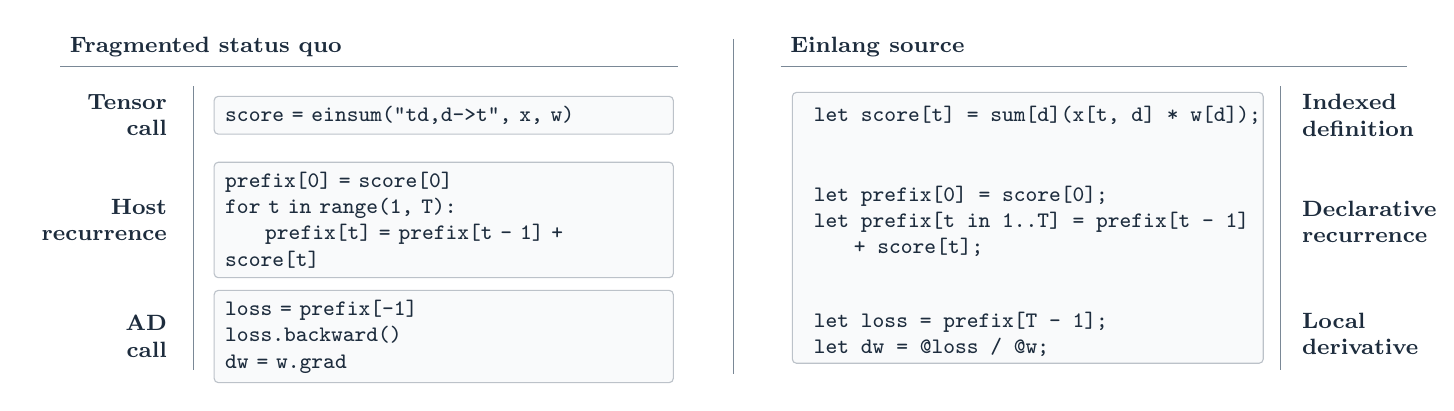
\begin{tikzpicture}[
  x=1cm,
  y=1cm,
  font=\footnotesize,
  code/.style={anchor=west, font=\ttfamily\footnotesize, text=figInk},
  codepart/.style={anchor=west, font=\ttfamily\footnotesize, text=figInk, align=left},
  codebox/.style={draw=einFrame, fill=einBg, rounded corners=1.5pt,
    line width=0.4pt, inner xsep=4pt, inner ysep=3.5pt,
    font=\ttfamily\footnotesize, text=figInk, align=left},
  sideleft/.style={anchor=east, font=\bfseries\footnotesize, text=figInk, align=right, text width=1.65cm},
  sideright/.style={anchor=west, font=\bfseries\footnotesize, text=figInk, align=left, text width=1.45cm},
  head/.style={anchor=west, font=\bfseries\footnotesize, text=figInk}
]
\node[head] at (0.00,3.20) {Fragmented status quo};
\node[head] at (9.15,3.20) {\einlang{} source};

\draw[draw=figLine, line width=0.4pt] (0.00,2.95) -- (7.85,2.95);
\draw[draw=figLine, line width=0.4pt] (9.15,2.95) -- (17.10,2.95);
\draw[draw=figLine, line width=0.35pt] (8.55,3.30) -- (8.55,-0.95);

% Left: split across separate host/API fragments.
\draw[draw=figLine, line width=0.35pt] (1.70,2.70) -- (1.70,-0.90);

\node[sideleft] at (1.48,2.33) {Tensor\\call};
\node[codebox, anchor=west, text width=5.55cm] at (1.95,2.33) {score = einsum(\figstr{"td,d->t"}, x, w)};

\node[sideleft] at (1.48,1.00) {Host\\recurrence};
\node[codebox, anchor=west, text width=5.55cm] at (1.95,1.00) {%
prefix[0] = score[0]\\
\figkw{for} t \figkw{in} range(1, T):\\
\hspace*{1.7em}prefix[t] = prefix[t - 1] + score[t]};

\node[sideleft] at (1.48,-0.48) {AD\\call};
\node[codebox, anchor=west, text width=5.55cm] at (1.95,-0.48) {%
loss = prefix[-1]\\
loss.backward()\\
dw = w.grad};

% Right: one co-resident source fragment.
\draw[draw=figLine, line width=0.35pt] (15.50,2.70) -- (15.50,-0.90);

\path[draw=einFrame, fill=einBg, rounded corners=1.5pt, line width=0.4pt]
  (9.30,-0.82) rectangle (15.28,2.62);
\node[codepart] at (9.45,2.33) {\figkw{let} score[t] = \figkw{sum}[d](x[t, d] * w[d]);};
\node[codepart] at (9.45,0.98) {%
\figkw{let} prefix[0] = score[0];\\
\figkw{let} prefix[t \figkw{in} 1..T] = prefix[t - 1]\\
\hspace*{1.7em}+ score[t];};
\node[codepart] at (9.45,-0.45) {%
\figkw{let} loss = prefix[T - 1];\\
\figkw{let} dw = \figad{@loss / @w};};
\node[sideright] at (15.65,2.33) {Indexed\\definition};

\node[sideright] at (15.65,0.98) {Declarative\\recurrence};

\node[sideright] at (15.65,-0.45) {Local\\derivative};

\end{tikzpicture}
\endgroup

\vspace{-0.35em}
\captionsetup{hypcap=false}
\caption{The design problem: the same mathematical structure is often split across host/API fragments for contraction, recurrence, and differentiation; \einlang{} keeps indexed definitions, recurrences, and derivative requests in one source language. Code-style highlighting follows the examples used throughout the paper.}
\Description{A comparison between a fragmented status quo with separate contraction, loop, and grad interfaces, and Einlang, where all three appear in a single source language. The code snippets use listing-style syntax coloring and boxes.}
\label{fig:fragmentation}
\vspace{-0.4em}
\end{figure*}

\subsection{Contributions and Focus}

We present \einlang{} as a language and compiler artifact. Its unit of contribution is an executable abstraction boundary: a source language that preserves useful tensor facts, plus the compiler and runtime machinery that consume those facts. Its contributions are:
\begin{itemize}
\item \textbf{Abstraction-boundary claim.} We identify indexed recurrence with local derivative queries as a productive source boundary for tensor programs that combine dynamic-programming, sequence, grid, and sensitivity structure.
\item \textbf{Unified source model.} We design a tensor language in which multidimensional indexed definitions, declarative recurrences, and local derivative requests share one binding environment.
\item \textbf{Compositional examples.} We show how the three constructs can be used independently, nested inside one another, and applied to intermediate values without wrapper-style refactoring.
\item \textbf{Compiler analysis example.} We describe how recurrent bindings induce multidimensional dependency graphs and how static offset vectors determine storage windows.
\item \textbf{Executable implementation.} We report on a NumPy-backed compiler and runtime with tests for numerical behavior, recurrence ordering/storage decisions, and lazy derivative projections.
\end{itemize}

The claims are intentionally scoped to what the artifact can demonstrate. Table~\ref{tab:claims-evidence} summarizes the correspondence between claim, mechanism, and evidence.

\begin{table*}[t]
\centering
\caption{Claims, mechanisms, and evidence for the current \einlang{} artifact.}
\label{tab:claims-evidence}
\renewcommand{\arraystretch}{1.08}
\setlength{\tabcolsep}{4pt}
\begin{tabular*}{\textwidth}{@{\extracolsep{\fill}}L{0.23\textwidth}L{0.34\textwidth}L{0.33\textwidth}@{}}
\toprule
Claim & Mechanism & Evidence \\
\midrule
Source coherence & Indexed definitions, recurrent clauses, and derivative requests share one binding environment. & Mixed examples combine contraction, recurrence, and derivative queries; source comparisons exercise the individual boundaries without wrapper-style refactoring. \\
Compiler leverage & Recurrent bindings preserve dependency offsets and later reads before lowering. & Storage checks distinguish finite suffix reads from full or dynamic observations. \\
Derivative locality & \texttt{@y/@x} is a shaped expression over named source bindings. & Julia/Zygote comparison and lazy derivative tests distinguish local derivative queries from function-boundary AD. \\
Executable breadth & A NumPy-backed compiler and runtime execute the language fragment used in the examples. & Reference-backed numerical checks, recurrence tests, and model-scale indexed programs exercise the implementation path. \\
Current boundary & Static-offset recurrence analysis infers one finite recurrence axis in the current compiler. & Multidimensional vector-window cases are stated as evaluation obligations rather than completed performance claims. \\
\bottomrule
\end{tabular*}
\end{table*}

The same positioning can be read feature by feature. Table~\ref{tab:feature-positioning} names the nearest neighboring interfaces for each source feature and states the corresponding \einlang{} advantage. The comparison is intentionally about the programming and compiler boundary, not about peak runtime performance. The later code figures make the table concrete for indexing, recurrence, and local derivatives; Section~\ref{sec:conv-comparison} does the same for convolution.

\begin{table*}[t]
\centering
\caption{Feature-by-feature source-interface positioning.}
\label{tab:feature-positioning}
\renewcommand{\arraystretch}{1.06}
\setlength{\tabcolsep}{4pt}
\begin{tabular*}{\textwidth}{@{\extracolsep{\fill}}L{0.20\textwidth}L{0.31\textwidth}L{0.23\textwidth}L{0.18\textwidth}@{}}
\toprule
\einlang{} feature & Nearby treatment in other systems & \einlang{} treatment & \einlang{} advantage \\
\midrule
Indexed reductions & \texttt{einsum} strings expose contraction; TVM and Halide expose compiler-facing tensor expressions and schedules. & Output axes, reduction axes, and affine reads are source-language names. & No contraction mini-language; axes stay in ordinary binding and scope. \\
Windowed convolution & \texttt{einsum} typically follows patch/window construction; TVM tensor expressions represent reductions and affine reads directly. & Convolution is one indexed binding with surviving axes, reduction axes, and offset reads. & Window offsets and contraction axes remain one source object before lowering. \\
Declarative recurrence & Host loops and JAX \texttt{scan} choose a loop/carry interface; Halide uses update definitions with schedules. & Base and recurrent clauses define dependencies over an index space. & Traversal, carry, and buffer choices can be delayed until compiler analysis. \\
Multidimensional recurrence storage & Scan nesting, manual line buffers, schedule directives, or lower-level dependence analysis manage storage. & Static self-read offsets and later observations induce storage windows. & Storage follows from source uses instead of user-selected buffers. \\
Local derivative requests & JAX and Julia/Zygote transform functions or pullbacks; PyTorch uses graph/backward state. & \texttt{@target/@wrt} is a shaped source expression over named bindings. & Intermediate sensitivities are local values, including inside recurrent programs. \\
Composition boundary & Mainstream systems compose these features through host-language APIs and transformation calls. & Indexing, recurrence, and derivatives share one checked binding environment. & Mixed tensor, recurrence, and AD code avoids wrapper-style refactoring. \\
\bottomrule
\end{tabular*}
\end{table*}

The evaluation follows from this framing: executable credibility, source comparisons against scan-style encodings, compiler metadata checks, local-derivative behavior, and model-scale feasibility.

The remainder of the paper is organized as follows. Section~2 gives motivating examples. Section~3 describes the language design. Section~4 describes recurrence analysis. Section~5 describes the implementation. Section~6 evaluates the design and its limits. Section~7 discusses related work, Section~8 discusses boundaries and extensions, and Section~9 concludes.

\section{Overview and Motivating Example}

We use one compact running example throughout the paper. It computes a per-timestep score, accumulates those scores through time, and differentiates the final result with respect to a weight vector:

\begin{lstlisting}[style=einlang]
let score[t] = sum[d](x[t, d] * w[d]);
let prefix[0] = score[0];
let prefix[t in 1..T] = prefix[t - 1] + score[t];
let loss = prefix[T - 1];
let dw = @loss / @w;
\end{lstlisting}

This compact example already exercises the three core abstractions. The notation \texttt{1..T} denotes the half-open range from \texttt{1} through \texttt{T-1}; the base clause defines \texttt{prefix[0]}, and the recurrent clause defines the remaining points.

\subsection{One Program, Three Semantic Objects}

The first line is an indexed tensor definition. It states directly that \texttt{score} is indexed by \texttt{t}, that \texttt{d} is reduced, and that the body is evaluated pointwise for each output index.

The next two lines form a declarative recurrence. The source says that \texttt{prefix[t]} depends on \texttt{prefix[t - 1]} and \texttt{score[t]}; loop order and storage strategy are compiler choices.

The final two lines add a local derivative request. The language first names the quantity of interest, \texttt{loss}, then asks for its derivative with respect to the named binding \texttt{w}. Differentiation is part of the same source program. What the compiler can read directly from this one program is already the point: the output axis \texttt{t}, the reduction axis \texttt{d}, the recurrence dependency \texttt{prefix[t - 1] -> prefix[t]}, and the differential target \texttt{loss / w} all remain visible in the same source fragment.

\subsection{Why This Example Matters}

In a library-oriented setting, the same task is usually split across an \texttt{einsum}-style interface or explicit tensor arithmetic, a host-language loop or scan combinator, and a \texttt{grad}/\texttt{backward}-style API. \einlang{} keeps the entire computation in one language. Its advantage is not merely shorter syntax; it is fewer semantic handoffs. The program reads more like the derivation the programmer had in mind, and the key tensor, recurrence, and differential facts remain structured through the compiler passes that consume them.

\subsection{Relation to Scan}

Staged scan operators are a good abstraction for many recurrent computations. They make loops transformable, usually interact well with AD, and can be optimized by mature compilers. A scan packages recurrence as an operator with an explicit carry, an update function, and an explicit decision about which intermediate values are returned.

The source question is different. Before choosing a schedule, a storage policy, or an AD transform boundary, the programmer may want to state that an indexed value is defined by a recurrence relation. In \einlang{}, the state sequence is a named binding, later expressions read points of that binding directly, and the compiler derives whether those reads require full materialization or only a finite suffix. A scan-oriented encoding can express the same computation, but the programmer must decide which values are carried, which outputs are stacked, and which intermediate values must be returned for later use. \einlang{} moves those decisions from the source interface into compiler analysis when the access pattern is statically visible.

\subsection{Comparison with PyTorch and JAX}

The same workload shape can be written in adjacent systems, including with staged recurrence operators such as \texttt{jax.lax.scan}. A direct JAX scan encoding is:

\noindent\begin{minipage}{\columnwidth}
\begin{lstlisting}[style=pythoncode]
def forward_scan(x, w):
    score = jnp.einsum("td,d->t", x, w)
    def step(acc, s):
        acc = acc + s
        return acc, acc
    _, prefix = jax.lax.scan(step, 0.0, score)
    return prefix[-1]

dw = jax.grad(lambda w, x: forward_scan(x, w))(w, x)
\end{lstlisting}
\end{minipage}

This is the right baseline for the running example: JAX exposes the recurrence to its staging machinery, and the gradient transform composes with the scan. The \einlang{} advantage is at the source interface. In JAX, the scan signature fixes a carry/output boundary before the compiler sees later uses of the sequence. In \einlang{}, the source defines \texttt{prefix[t]} as an indexed recurrent binding; later reads such as \texttt{prefix[T-1]} are ordinary source reads that the storage analysis can inspect before choosing a circular buffer or full materialization.

\section{Language Design}

\subsection{Design Principle: Orthogonal Abstractions}

\einlang{} is organized around a simple design principle: each major source of structure in differentiable tensor programs should correspond to one direct language construct, and those constructs should compose without semantic gaps. We use three constructs as the language's small vocabulary:
\begin{itemize}
\item \textbf{index space}: which axes are output axes, and which are reduced;
\item \textbf{dependency structure}: how values evolve across a range; and
\item \textbf{differential structure}: which named quantities require sensitivities.
\end{itemize}

This is why the language centers on indexed definitions, recurrences, and derivative requests rather than on helper conventions layered over a generic host language. Each construct has an interface contract: it introduces names, determines shapes, and states what later compiler phases may rely on.

\subsection{Clause-Scoped Index Domains}

Indexed tensor definitions are the basic connective tissue of the language:

\begin{lstlisting}[style=einlang]
let C[i, j] = sum[k](A[i, k] * B[k, j]);
\end{lstlisting}

Here \texttt{i} and \texttt{j} are output indices and \texttt{k} is a reduction index. The source tells the reader and the compiler which axes survive into the result and which axes are contracted away.

\paragraph{Contract.}
For a binding
\[
\texttt{let } X[i_1 \in R_1,\ldots,i_k \in R_k] = e,
\]
the clause covers the index domain $R_1 \times \cdots \times R_k$. Index variables are lexically scoped: an output index is available only in the right-hand side of its binding, a reduction index introduced by \texttt{sum} is available only inside that reduction body, and inner index declarations may shadow outer names. Index variables do not escape into later bindings. A name that appears in the output index list denotes an output axis; an index introduced only inside a reduction denotes an axis that is consumed by that reduction.

\paragraph{Clause coverage.}
A tensor binding may be assembled from multiple clauses, written as surface \texttt{let} statements with the same left-hand-side name. Each clause defines only the points in its own domain, so one statement can define a boundary slice such as \texttt{D[0, j in 0..N]} while another defines an interior region such as \texttt{D[i in 1..M, j in 1..N]}. Semantically, the binding's covered domain is the union of these clause domains. The compiler preserves this fact when grouping clauses; for rectangular array backends, it allocates the per-axis extent that contains the covered domain. This lets different statements define different parts of one tensor without treating every statement as a full-tensor definition.

\paragraph{Range elaboration.}
The surface language permits index ranges to be written explicitly or omitted when shaped tensor accesses determine them. Range elaboration is the front-end normalization step that makes this precise: before shape analysis, the compiler builds an index environment and attaches an explicit range object to each index variable when it can. A source declaration such as \texttt{i in 0..N} contributes that range directly. Otherwise, an occurrence of an index variable in axis $a$ of a tensor with shape $S$ contributes the candidate range $0..S_a$; for example, \texttt{A[i,k]} contributes the first-axis range for \texttt{i} and the second-axis range for \texttt{k}. Reduction indices are elaborated in the same way, but only inside the reduction body. Simple affine forms such as \texttt{i+1} or \texttt{i-r} are checked against the elaborated axis bounds when the offset is statically bounded. If several uses constrain the same index, the compiler intersects the candidate ranges. If no usable range can be recovered, later passes either require a source range or use a conservative path such as full materialization for recurrence storage.

This differs from string-based contraction APIs. A call such as \texttt{einsum("ik,kj->ij", ...)} exposes the right mathematical idea, but it does so through a separate mini-language. In \einlang{}, the indexed structure participates in the ordinary scope, analysis, and error-reporting mechanisms of the language itself. The advantage is not that every contraction is fewer characters than \texttt{einsum}; the advantage is that the axes remain named source facts that can be checked, reused, and composed with recurrence and derivative requests. Compiler-oriented systems such as TVM and Halide make tensor or image expressions available to powerful scheduling stacks \cite{tvm2018,halide2013}. \einlang{} does not replace those scheduling interfaces; its point is earlier in the pipeline, where the indexed relation is still a source binding rather than a scheduled operator. Figure~\ref{fig:index-code-comparison} shows the same matrix multiplication boundary in the nearby notations.

\begin{figure}[t]
\centering
\begin{minipage}[t]{0.98\linewidth}
\textbf{\einlang{}}
\begin{lstlisting}[style=einlang]
let C[i, j] = sum[k](A[i, k] * B[k, j]);
\end{lstlisting}
\end{minipage}

\vspace{0.25\baselineskip}
\begin{minipage}[t]{0.98\linewidth}
\textbf{NumPy \texttt{einsum}}
\begin{lstlisting}[style=pythoncode]
C = np.einsum("ik,kj->ij", A, B)
\end{lstlisting}
\end{minipage}

\vspace{0.25\baselineskip}
\begin{minipage}[t]{0.98\linewidth}
\textbf{TVM tensor expression}
\begin{lstlisting}[style=pythoncode]
k = te.reduce_axis((0, K), "k")
C = te.compute((M, N), lambda i, j: te.sum(
    A[i, k] * B[k, j], axis=k))
\end{lstlisting}
\end{minipage}

\vspace{0.25\baselineskip}
\begin{minipage}[t]{0.98\linewidth}
\textbf{Halide update}
\begin{lstlisting}[style=pythoncode]
Var i, j;
RDom k(0, K);
Func C;
C(i, j) += A(i, k) * B(k, j);
\end{lstlisting}
\end{minipage}
\caption{Indexed reduction in adjacent source interfaces. The computation is the same; the boundary exposed to later compiler phases differs.}
\label{fig:index-code-comparison}
\end{figure}

Shape checking follows the same scoping discipline. A tensor read must provide one subscript expression for each tensor axis. Subscript expressions that mention index variables must be statically range-checkable in the current index environment. The compiler accepts affine offset forms such as \texttt{i}, \texttt{i+1}, and \texttt{i-2}; dynamic offsets are rejected for static indexing analysis or force conservative storage decisions when they appear in recurrent self-reads. This is the substitution rule for index programs: a point of an indexed binding is obtained by substituting concrete values for the in-scope output indices and then evaluating the body under those bindings.

\paragraph{Broadcasting.}
\einlang{} uses an explicit broadcasting rule. Scalars are implicitly broadcast. Non-scalar tensors are indexed explicitly, and broadcasting over an output dimension is expressed by omitting that output index from a particular indexed read. For example:
\begin{lstlisting}[style=einlang]
let Y[i in 0..M, j in 0..N] = row[i] + col[j] + bias;
\end{lstlisting}
Here \texttt{row[i]} is invariant in \texttt{j}, \texttt{col[j]} is invariant in \texttt{i}, and scalar \texttt{bias} is broadcast over both output axes. This rule keeps broadcasting visible in the same index environment as ordinary tensor reads.

The full language also includes minor surface conveniences, such as named rest indices written with syntax like \texttt{..batch}; the core abstraction remains clause-scoped indexed binding.

\subsection{Declarative Recurrence}

Many tensor-heavy programs are naturally written as recurrence relations:

\begin{lstlisting}[style=einlang]
let x[0] = x0;
let x[t in 1..T] = step(x[t - 1], u[t]);
\end{lstlisting}

The important point is that this is a declaration of dependency. The programmer states what depends on what; the compiler later derives a legal execution order. This design is especially relevant for dynamic programming, autoregressive decoding, iterative optimization, ODE-style time stepping, and similar workloads in which mathematical recurrence is central.

\paragraph{Contract.}
A recurrent binding may be defined by multiple clauses: base clauses supply boundary points, and recurrent clauses define the remaining domain. Inside a recurrent clause, the right-hand side may read other points of the same binding. Such a self-read is statically analyzable when its subscripts are the current recurrence indices plus constant offsets. The compiler's obligation is then simple: evaluate each point after the points it reads have been produced. Programs outside this static fragment use the full materialization path described in Section~6. The source program specifies dependencies; the compiler chooses a legal traversal.

The same syntax applies to multidimensional recurrence:
\begin{lstlisting}[style=einlang]
let H[0, j in 0..N] = top[j];
let H[i in 0..M, 0] = left[i];
let H[i in 1..M, j in 1..N] =
    mix(H[i - 1, j], H[i, j - 1], input[i, j]);
\end{lstlisting}
The recurrence domain is now a grid, and the source exposes a dependency relation over grid points rather than a single scan axis. By keeping recurrence as a source construct, \einlang{} gives the compiler a semantic object to analyze. Dependency information is available before lowering, so recurrence ordering and storage choices can be derived from source meaning rather than reconstructed from already lowered loops.

Compared with a scan interface such as JAX \texttt{lax.scan}, the recurrent binding does not ask the programmer to choose a carry state or stacked output contract up front. Compared with update-style DSLs and schedule-oriented systems, the recurrent binding is not primarily a performance schedule; it is the source dependency object from which traversal and storage plans are derived. The \einlang{} advantage is delayed commitment: source code states the recurrence relation, while the compiler derives the legal order and storage plan from the observed reads. Figure~\ref{fig:recurrence-code-comparison} shows the difference at the source level.

\begin{figure}[t]
\centering
\begin{minipage}[t]{0.98\linewidth}
\textbf{\einlang{}}
\begin{lstlisting}[style=einlang]
let y[0] = init;
let y[t in 1..T] = step(y[t - 1], x[t]);
let out = y[T - 1];
\end{lstlisting}
\end{minipage}

\vspace{0.25\baselineskip}
\begin{minipage}[t]{0.98\linewidth}
\textbf{JAX \texttt{scan}}
\begin{lstlisting}[style=pythoncode]
def body(carry, x_t):
    y = step(carry, x_t)
    return y, y
out, ys = jax.lax.scan(body, init, x[1:])
out = ys[-1]
\end{lstlisting}
\end{minipage}

\vspace{0.25\baselineskip}
\begin{minipage}[t]{0.98\linewidth}
\textbf{PyTorch host loop}
\begin{lstlisting}[style=pythoncode]
ys = [init]
for x_t in x[1:]:
    ys.append(step(ys[-1], x_t))
out = ys[-1]
\end{lstlisting}
\end{minipage}
\caption{One-step recurrence in adjacent source interfaces. JAX and PyTorch expose the loop/carry/list decision directly; \einlang{} exposes the dependency relation.}
\label{fig:recurrence-code-comparison}
\end{figure}

\subsection{Local Derivative Requests}

Differentiation in \einlang{} is requested locally:

\begin{lstlisting}[style=einlang]
let dloss_dW = @loss / @W;
\end{lstlisting}

This places differentiation at the expression level rather than only at a function boundary, as in many AD frameworks \cite{tensorflow2016,pytorch2019,jax2018,baydin2018}. The derivative request appears where the derivative is needed, over the named program bindings already present in the source. The full surface language also includes bare tangent requests such as \texttt{@x}; the quotient form is the main vehicle for source-level derivative queries.

\paragraph{Contract.}
The expression \texttt{@y / @x} denotes a shaped derivative object. If \texttt{y} is scalar and \texttt{x} has shape $S_x$, the result has shape $S_x$. If both are tensors, the result shape combines target and parameter axes, and projections such as \texttt{(@y/@x)[i,j]} select derivative entries. A derivative request is a pure query over the existing source environment, and lowering is responsible for replacing that query with an executable derivative representation.

The important design choice is locality. A derivative request may target an intermediate indexed or recurrent binding, not only the final result of a function boundary:
\begin{lstlisting}[style=einlang]
let h[0, j] = h0[j];
let h[t in 1..T, j] = cell(h[t - 1, j], x[t, j], theta[j]);
let local[t, j] = @h[t, j] / @theta[j];
let score = sum[t, j](mask[t] * local[t, j]);
\end{lstlisting}
In a wrapper-oriented interface, this pattern usually forces the programmer to carve out a separate differentiable function or expose intermediate states as auxiliary returns. In \einlang{}, the derivative is an expression over bindings that already exist in the indexed source program.

This local style is useful for intermediate sensitivities, custom optimization steps, and mixed workloads in which only part of a larger recurrent or numerical program needs differentiation. It is also useful to the compiler: the target binding, parameter binding, output shape, parameter shape, and surrounding recurrence structure are all still represented when the request is lowered.

The local request can also appear inside a recurrent definition. The following program performs gradient descent on the scalar objective $x^2$ while keeping each optimization step as a recurrent source binding:
\begin{lstlisting}[style=einlang]
let alpha = 0.25;
let x[0] = 8.0;
let x[k in 1..6] = {
    let prev = x[k - 1];
    let loss = prev * prev;
    let g = @loss / @prev;
    prev - alpha * g
};
\end{lstlisting}
Here the derivative target \texttt{prev} is a block-local name introduced inside the recurrent body. A function-oriented AD interface can express the same update by carving out an update function and applying a transform to it; \einlang{} expresses the derivative at the point where the mathematical update is written. This is the intended role of local differentiation in the paper: a source-level derivative expression that composes with indexed and recurrent bindings.

\paragraph{Lowering algorithm.}
The compiler treats \texttt{@y/@x} as a local Jacobian query, not as a request to transform the enclosing function. After type and shape analysis, the autodiff pass recognizes quotient forms whose numerator and denominator are differentials of named bindings, records the target/wrt pair, and snapshots the source bindings and block-local contexts needed to re-evaluate the selected expression. It then rewrites the quotient to a \texttt{LazyJacobianIR(target,wrt)} node. A later request-lowering pass removes that node before backend execution. If the lazy Jacobian is projected, as in \texttt{J[i,j]} or \texttt{(@y/@x)[i,j]}, the pass fuses the projection: a fixed target index lowers to a VJP row query with a basis cotangent, while a fixed parameter index may lower to a JVP column query with a basis tangent. If the whole Jacobian is demanded, the pass materializes it as an indexed binding over target axes followed by parameter axes, choosing JVP or VJP by a static size heuristic. This is the smart part of local expression AD: the user writes a shaped local value, while the compiler delays the row/column/full decision until it sees how that value is consumed.

\paragraph{Comparison with Julia-style expression AD.}
Julia is an important positive baseline because systems such as Zygote differentiate ordinary Julia programs with source-to-source AD \cite{julia2017,zygote2019}. The user can keep scientific code in the host language, but the derivative boundary is still usually a function, closure, or pullback. Figure~\ref{fig:ad-code-comparison} shows the same local sensitivity request across the nearby interfaces. \einlang{} deliberately gives up host-language generality to gain a sharper tensor-language boundary: the tensor program is written in an indexed source language, and the local sensitivity remains an expression over names already in that language. The advantage is therefore not that Julia/Zygote, JAX, or PyTorch cannot compute the derivative; they can. The advantage is that \einlang{} places the derivative request where the selected intermediate is defined and used, so intermediate and recurrent sensitivities need not be repackaged behind a function boundary.

\begin{figure}[t]
\centering
\begin{minipage}[t]{0.98\linewidth}
\textbf{\einlang{}}
\begin{lstlisting}[style=einlang]
let local[t, j] = @h[t, j] / @theta[j];
\end{lstlisting}
\end{minipage}

\vspace{0.25\baselineskip}
\begin{minipage}[t]{0.98\linewidth}
\textbf{JAX function transform}
\begin{lstlisting}[style=pythoncode]
local = jax.grad(lambda theta: run(theta)[t, j])(theta)[j]
\end{lstlisting}
\end{minipage}

\vspace{0.25\baselineskip}
\begin{minipage}[t]{0.98\linewidth}
\textbf{Julia/Zygote source AD}
\begin{lstlisting}[style=pythoncode]
using Zygote
local = gradient(theta -> run(theta)[t, j], theta)[1][j]
\end{lstlisting}
\end{minipage}

\vspace{0.25\baselineskip}
\begin{minipage}[t]{0.98\linewidth}
\textbf{PyTorch backward}
\begin{lstlisting}[style=pythoncode]
h = run(theta)
theta.grad = None
h[t, j].backward(retain_graph=True)
local = theta.grad[j]
\end{lstlisting}
\end{minipage}
\caption{Local derivative request in adjacent source interfaces. Host AD systems package the selected value behind a function, pullback, or graph state; \einlang{} keeps the sensitivity as a shaped source expression.}
\label{fig:ad-code-comparison}
\end{figure}

\paragraph{AD interface trade-offs.}
Expression-level derivative requests occupy a different point in the AD interface design space from whole-function transforms, source-to-source host-language AD, and tape-style backward calls. Table~\ref{tab:ad-design-space} summarizes the trade-off. JAX-style transforms make the differentiated function boundary explicit, which is excellent for caching and higher-order transformation, but intermediate sensitivities usually require returning auxiliary values or defining additional transformed functions. Julia/Zygote keeps that boundary inside an expressive host language, which is powerful for scientific programs, while still asking the user to identify a function or pullback boundary for a derivative query. PyTorch-style backward calls are flexible in an imperative program, but gradients are mediated by side effects on tensors and gradient buffers. \einlang{} makes a derivative request an expression over named source bindings. Its advantage appears when a program asks for several shaped sensitivities inside the same indexed or recurrent computation, such as both \texttt{@loss/@theta} and \texttt{@h[t]/@theta}. The cost is a compiler obligation: the compiler must track target/wrt dependencies, avoid leaking source AD artifacts after lowering, and decide when multiple derivative requests should share work.

\begin{table*}[t]
\centering
\caption{AD interface design space relevant to local derivative requests.}
\label{tab:ad-design-space}
\renewcommand{\arraystretch}{1.08}
\setlength{\tabcolsep}{3pt}
\begin{tabular*}{\textwidth}{@{\extracolsep{\fill}}L{0.16\textwidth}L{0.25\textwidth}L{0.24\textwidth}L{0.25\textwidth}@{}}
\toprule
Interface & Strength & Cost & Consequence for intermediates \\
\midrule
Whole-function transform & Clear transform boundary; reusable compiled derivative. & Programmer packages the computation as a function. & Intermediate derivatives require auxiliary returns or additional transforms. \\
Julia/Zygote source AD & Differentiates rich host-language programs. & Derivative query is still organized around a function, closure, or pullback. & Intermediate derivatives require wrapping the selected value or seeding a pullback. \\
Tape/backward call & Natural in imperative host code. & Gradient state is managed through side effects. & Intermediate gradients depend on retained graph state and buffer management. \\
Expression-level request & Derivative is a typed source expression over named bindings. & Compiler must lower and schedule multiple requests carefully. & Intermediate and recurrent sensitivities can be requested where they are used. \\
\bottomrule
\end{tabular*}
\end{table*}

Local derivative syntax makes the source query precise; cross-request reuse then becomes a compiler optimization problem. When two requests share a large primal subcomputation, a whole-function AD system with a carefully chosen transform boundary may reuse more work. \einlang{} improves source locality and access to intermediate sensitivities, while leaving cross-request derivative optimization as part of the implementation roadmap.

\subsection{Compositionality and Closure}

The main language claim appears when the three constructs interact. A tensor program may need a derivative of a recurrent quantity, an indexed derivative object, or a batch-polymorphic recurrent update. In \einlang{}, these are still source-language programs rather than combinations of separate APIs.

That closure matters because real workloads rarely stop at just one construct. A program often begins as an indexed equation, then acquires recurrence, then needs one or more local derivative queries. A stable source model is more valuable than three isolated conveniences.

Representative combinations all stay inside the same source model: a local derivative of one indexed contraction such as \texttt{@(sum[k](A[i,k] * B[k,j])) / @A[p,q]}, a recurrent sensitivity such as \texttt{@x[T] / @x[0]}, or the full indexed-recurrent-differentiable form \texttt{@loss / @w} from the running example. This is the design point: the constructs share binding, range, and shape information before lowering.

\section{Compiler Analysis for Recurrence}

This section describes the compiler analysis that recurrence exposes. The analysis shows how the language design gives the compiler useful structure for ordering and storage planning, especially when a recurrence ranges over more than one index dimension.

\subsection{Shape and Index Consistency}

Before extracting recurrence dependencies, the compiler builds an index environment from each binding. This is the evaluator's bookkeeping layer. Each clause contributes the output ranges or literal subscripts for the region it covers; grouping clauses by binding name gives the binding's covered domain, and rectangular backends use the corresponding per-axis allocation extent. Reduction ranges contribute only to the body they bind, and block-local index variables do not escape. A tensor read must supply a subscript for every axis of the tensor being read. The read shape is scalar at the point of use, while omitted output indices in the surrounding expression indicate explicit broadcast over those output dimensions, as described in Section~3.

Static recurrence analysis requires subscript expressions to be simple enough to compare against elaborated clause domains. The fragment used for storage analysis accepts an index variable plus or minus an integer constant. This makes two checks mechanical: the compiler can require a base clause for out-of-range boundary reads, and it can turn each self-read into an offset vector. More general expressions remain expressible and use full storage unless a later analysis proves a static bound.

\subsection{Extracting Multidimensional Dependencies}

To understand a recurrence, we ask one question: which previously computed points does this point need? A recurrent binding is a named indexed definition whose right-hand side reads the same binding at other index points. For a recurrent clause
\[
B = \texttt{let } y[i_1 \in R_1,\ldots,i_k \in R_k] = e,
\]
the compiler treats each point in $R_1 \times \cdots \times R_k$ as a graph node. It then looks at the right-hand side exactly as a reader would: every occurrence of \texttt{y} is a dependency. A self-read is statically analyzable when each subscript has the form $i_d + c_d$ where $c_d$ is an integer constant. The read then contributes an offset vector
\[
\delta = (c_1,\ldots,c_k).
\]
For the grid recurrence
\begin{lstlisting}[style=einlang]
let D[i in 1..M, j in 1..N] =
    min(D[i - 1, j], D[i, j - 1], D[i - 1, j - 1]);
\end{lstlisting}
there are three self-references. The first says that \texttt{D[i,j]} needs the point one step back in the \texttt{i} direction. The second says it needs the point one step back in the \texttt{j} direction. The third says it needs the diagonal predecessor. The extracted offsets are therefore $(-1,0)$, $(0,-1)$, and $(-1,-1)$.

The finite-window analysis uses only offsets with static bounds. A read such as \texttt{D[i-r, j]} uses full storage unless the compiler has a static bound for \texttt{r}. Boundary clauses are checked separately: base cases such as \texttt{D[0,j]} and \texttt{D[i,0]} establish the values needed before the recursive grid interior is evaluated. Shape checking ensures that every indexed read supplies a subscript for every axis and that statically analyzable offsets stay inside the elaborated clause domains or are guarded by a base clause.

For each dimension $d$, the analysis computes the maximum backward distance
\[
h_d = \max(0,\ -\min_{\delta \in \Delta_B} \delta_d),
\]
where $\Delta_B$ is the set of extracted self-read offset vectors. Positive offsets indicate forward dependencies and call for a different schedule. A legal schedule is any topological order of the resulting point graph. For the common lexicographic grid cases in this paper, the extracted offsets are non-positive in the recurrence dimensions, so row-major or timestep-major execution is legal after boundary clauses have been checked.

\subsection{Storage Window Inference}

The same recurrent binding can often be evaluated without storing the whole tensor. Consider first the one-dimensional recurrence \texttt{x[t] = x[t-1] + x[t-2]}. When the evaluator is producing \texttt{x[t]}, it needs the two most recent previous values. After it writes \texttt{x[t]}, that new value becomes part of the history needed by future steps. Thus a lookback of two requires a preservation window of three: the current value plus the two previous values that future bodies may read.

Later source reads add a second requirement. If the rest of the program reads only \texttt{x[T-1]}, then after the recurrence finishes it needs only the final suffix of length one. If it reads the last five points, it needs suffix length five. The compiler chooses a window large enough for both the recurrence body and the later observations.

The implemented compiler emits a finite window for one inferred recurrence dimension; that rule is the scalar case of a vector-window rule. For each recurrence dimension $d$, the analysis computes:
\begin{itemize}
\item \textbf{lookback} $h_d$: the largest static backward self-read distance in dimension $d$;
\item \textbf{tail} $s_d$: the largest statically visible final suffix read by later code in dimension $d$; and
\item \textbf{full}: whether later code may observe an arbitrary element or the whole recurrent value.
\end{itemize}
When no full observation is required, the preservation window for each finite dimension is
\[
w_d = \max(h_d+1,s_d).
\]
The $+1$ is the current point. Without it, the buffer would hold the previous history but not the newly produced value that later points will read. The resulting buffer shape is
\[
(w_1,\ldots,w_k),
\]
with $w_d=\infty$ for dimensions that are retained fully. Thus a dynamic program may use a buffer shaped like $(2,N)$: a sliding pair of rows and all columns. Dynamic self-reads and dynamic later reads use the full materialization path for the affected binding or dimension.

\paragraph{Intuitive correctness argument.}
Windowed execution is equivalent to full materialization whenever two conditions hold: every self-read needed while computing a point is still in the buffer, and every later program-visible read is either in the retained suffix or the whole value has been materialized. The vector rule above is a sufficient condition for those two facts because each dimension retains enough history for the largest static backward offset and enough suffix for later observations. The finite-window path is enabled exactly when the inferred window covers the visible reads.

\subsection{What This Buys}

The storage rule illustrates the value of making recurrence a named source binding over an index space. In a host-loop program, the programmer usually commits to appending, stacking, or line-buffering before later uses are known to the compiler. In \einlang{}, later reads of the recurrent binding remain source-level uses. The compiler can inspect those uses before deciding whether to allocate a finite window or a full array.

The current NumPy backend uses this metadata to choose a buffer strategy for recurrence tests, making storage planning a consequence of the source abstraction.

\section{Implementation}

\subsection{Compiler Architecture}

\einlang{} is implemented as a Python-embeddable compiler and runtime. The main executable path uses the NumPy backend, with an experimental IREE path as an additional backend direction. The compiler is structured to preserve source-level tensor, recurrence, and differential structure long enough for the analyses and transformations that depend on them. This section is organized around the implementation discipline behind the design claim: indexed recurrence gives the compiler a source dependency object before lowering.

\begin{figure*}[t]
\centering
\resizebox{0.88\textwidth}{!}{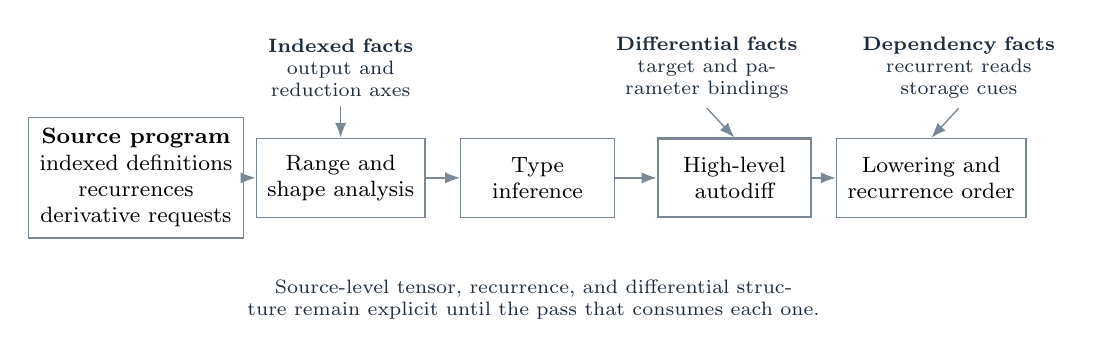
\begin{tikzpicture}[
  x=1cm,
  y=1cm,
  >=Latex,
  font=\footnotesize,
  stage/.style={draw=figLine, line width=0.5pt, minimum width=1.95cm, minimum height=1.0cm, align=center, inner sep=4pt},
  source/.style={draw=figLine, line width=0.55pt, minimum width=2.55cm, minimum height=1.15cm, align=center, inner sep=4pt},
  highlight/.style={stage, line width=0.75pt},
  fact/.style={font=\scriptsize, align=center, text=figInk, text width=2.45cm},
  line/.style={-{Latex[length=1.9mm]}, draw=figLine, line width=0.5pt}
]
\node[source] (src) at (1.45,0.75) {%
\textbf{Source program}\\
indexed definitions\\
recurrences\\
derivative requests};
\node[stage] (s1) at (4.05,0.75) {Range and\\shape analysis};
\node[stage] (s2) at (6.55,0.75) {Type\\inference};
\node[highlight] (s3) at (9.05,0.75) {High-level\\autodiff};
\node[stage] (s4) at (11.55,0.75) {Lowering and\\recurrence order};

\draw[line] (src.east) -- (s1.west);
\draw[line] (s1.east) -- (s2.west);
\draw[line] (s2.east) -- (s3.west);
\draw[line] (s3.east) -- (s4.west);

\node[fact] (f1) at (4.05,2.15) {\textbf{Indexed facts}\\output and reduction axes};
\node[fact] (f2) at (8.70,2.15) {\textbf{Differential facts}\\target and parameter bindings};
\node[fact] (f3) at (11.90,2.15) {\textbf{Dependency facts}\\recurrent reads\\storage cues};

\draw[line] (f1.south) -- (s1.north);
\draw[line] (f2.south) -- (s3.north);
\draw[line] (f3.south) -- (s4.north);

\node[font=\scriptsize, text=figInk, align=center, text width=11.7cm] at (6.50,-0.80)
{Source-level tensor, recurrence, and differential structure remain explicit until the pass that consumes each one.};
\end{tikzpicture}
}
\vspace{-0.35em}
\captionsetup{hypcap=false}
\caption{Compiler staging: indexed, recurrent, and derivative facts are preserved until the high-level passes that consume them.}
\Description{A diagram showing indexed and differential facts from the source flowing through tensor IR, range and shape analysis, type inference, high-level autodiff, and lowering.}
\label{fig:pipeline}
\vspace{-0.4em}
\end{figure*}

The implementation follows a single discipline: source facts are preserved until the pass that can use them has run. Indexed definitions survive long enough for range and shape analysis to distinguish output axes from reduction axes. Derivative requests survive long enough to be checked against named source bindings and lowered into lazy derivative objects. Recurrent bindings survive long enough for the compiler to inspect self-reads and later reads before selecting an execution order or storage policy. Table~\ref{tab:compiler-invariants} summarizes this preservation chain.

\begin{table*}[t]
\centering
\caption{Compiler phases and the source facts they preserve or consume.}
\label{tab:compiler-invariants}
\renewcommand{\arraystretch}{1.08}
\setlength{\tabcolsep}{4pt}
\begin{tabular*}{\textwidth}{@{\extracolsep{\fill}}L{0.20\textwidth}L{0.40\textwidth}L{0.30\textwidth}@{}}
\toprule
Phase & Preserved fact & Consumed by \\
\midrule
Source IR & output axes, reduction axes, clause domains, binding names & range and shape analysis \\
Typed IR & binding shapes and index ranges & derivative shape checks, recurrence checks \\
AD lowering & target/wrt binding pair, local contexts & request lowering to plain tensor IR \\
Recurrence ordering & self-read offsets and later reads & execution order, storage window \\
\bottomrule
\end{tabular*}
\end{table*}

\subsection{IR and High-Level Passes}

The front end preserves indexed bindings, recurrence declarations, and derivative requests as structured nodes through the passes that consume them. This makes range analysis and shape analysis source-directed. Because output axes and reduction axes remain source-level names, shape reasoning operates over the same structure the programmer wrote. Because derivative requests refer to named bindings, autodiff requests can be lowered before the tensor program has been flattened into execution-level detail.

One important consequence is phase discipline. The implementation includes both pre- and post-autodiff pruning passes as well as an autodiff leak check that fails if source-level differential artifacts survive into later stages unexpectedly. This makes derivative requests part of the compiler pipeline instead of a wrapper applied outside the source language.

At a design level, the implementation therefore preserves the same three semantic objects emphasized in the language section: indexed tensor structure, recurrence structure, and derivative requests. The concrete IR class names are less important than that preservation property. The compiler continues to know which axes are outputs versus reductions, which bindings are recurrent and with what storage requirements, and which named sensitivities are being requested.

For example, the source-level program
\begin{lstlisting}[style=einlang]
let s[0] = x0;
let s[t in 1..T] = f(s[t-1], u[t]);
let grad = @s[T] / @x0;
\end{lstlisting}
retains both recurrence metadata and the local derivative request until the passes that consume them. Recurrence ordering sees the indexed self-dependency, while derivative-request lowering turns the sensitivity query into a lazy derivative object with the source target and parameter still recorded.

\subsection{Recurrence Ordering}

Recurrence is handled by a dedicated ordering pass that derives valid execution order from dependency structure. In the simple running example this is straightforward, and the same mechanism extends to more complicated recurrence objects, including cases where clause structure requires timestep-major execution to preserve same-step dependencies. The same pass records storage metadata for isolated recurrences: history lookback, downstream tail use, whether full output must be preserved, and a derived \texttt{preserve\_steps} window. The current NumPy backend uses that metadata to switch to circular-buffer execution when bounded history and bounded tail reads make full materialization unnecessary.

The storage analysis deliberately errs toward full materialization. Static backward offsets and statically visible tail reads contribute to the preservation window. If a later use may inspect an arbitrary element, export the whole recurrent value, or otherwise escape the finite-window invariant, the pass marks the recurrence as requiring full output. This is the implementation counterpart of the storage invariant in Section~4.

The pass emits storage facts for backend code. Its output records whether a binding is recurrent, the recurrence dimension, ordering constraints between recurrent clauses, the maximum static lookback, the later suffix demand, and the final full-versus-windowed storage decision. The NumPy backend consumes those facts later; other backends can make a different scheduling choice while respecting the same source-level storage contract.

The important implementation detail is that the storage decision is made before backend-specific execution code is emitted. At that point the compiler still has three pieces of source information together: the recurrent binding name, the self-read offsets inside the recurrent clause, and the later reads of that binding in the ordered program. After lowering to an ordinary loop over a mutable buffer, this information would be partly implicit in control flow and partly implicit in host data-structure choices. Keeping recurrence as a source construct therefore changes the compiler problem from recovering a loop idiom to checking a finite-window condition over source reads.

\begin{table*}[t]
\centering
\caption{Storage-planning outcomes for recurrent bindings.}
\label{tab:storage-outcomes}
\renewcommand{\arraystretch}{1.08}
\setlength{\tabcolsep}{6pt}
\begin{tabular}{@{}lll@{}}
\toprule
Observed source pattern & Compiler fact & Backend consequence \\
\midrule
Static backward self-reads only & finite lookback $h$ & circular-buffer candidate \\
Later reads confined to final suffix & finite tail $s$ & retain suffix in same buffer \\
Whole-tensor or dynamic later read & $\mathit{full}(B)$ & materialize full sequence \\
Same-step dependency across clauses & ordering constraint & timestep-major schedule \\
\bottomrule
\end{tabular}
\end{table*}

This pass is not only an implementation detail; it exercises the language choice to make recurrence declarative. The compiler can derive both execution order and concrete storage choices for recurrence because the source describes dependencies directly.

\subsection{Circular Buffers and the Multidimensional Extension}

The circular-buffer runtime stores a logical tensor in a smaller physical array by applying modulo translation to each finite-window dimension. With row-major strides, a logical point maps to
\[
\mathit{offset} =
\sum_d ((i_d \bmod w_d) \cdot \mathit{stride}_d),
\]
where dimensions with $w_d=\infty$ use the ordinary full coordinate instead of a circular coordinate. Boundary clauses initialize the frontier needed by the first interior points; interior evaluation then overwrites buffer slots only after all future reads of the old point have passed.

The current NumPy backend exercises this path for multidimensional tensor values whose finite window is on the primary recurrence axis, for example a buffer shaped $(2,N)$ instead of $(T,N)$. The same buffer abstraction accepts finite windows on multiple axes; extending inference and scheduling to general mixed finite/full vector windows is the next implementation step.

\subsection{Autodiff Request Lowering}

The implementation separates source recognition from backend execution. \texttt{AutodiffPass} runs after type, shape, and pre-autodiff pruning. It records the source binding graph and block-local binding contexts, rewrites quotient requests over identifiers to \texttt{LazyJacobianIR}, and expands bare differentials. \texttt{AutodiffRequestLoweringPass} then lowers derivative requests to ordinary tensor IR. A leak-check pass ensures that no autodiff-only IR reaches later lowering.

Request lowering is consumption-sensitive. If a named lazy Jacobian is only used through rectangular accesses, the binding can be removed and each use is rewritten directly. Row projections lower to VJP-style code with a basis cotangent; column projections lower to JVP-style code with a basis tangent; full materialization emits an indexed tensor whose axes are target axes followed by parameter axes. The pass chooses between JVP and VJP using static target/wrt sizes when available. The separate \texttt{LazyJacobianValue} runtime object exercises the same row/column/entry interface in tests, but the normal NumPy backend path receives plain IR after request lowering.

\begin{table}[t]
\centering
\caption{Observable local-derivative query forms.}
\label{tab:derivative-queries}
\renewcommand{\arraystretch}{1.08}
\small
\setlength{\tabcolsep}{4pt}
\begin{tabular}{@{}lll@{}}
\toprule
Use & Shape & Lowered query \\
\midrule
\texttt{@y / @x} & $\sigma_y \times \sigma_x$ & materialized only if demanded \\
\texttt{(@y/@x)[a,b]} & scalar & entry via JVP or VJP \\
\texttt{(@y/@x)[a,:]} & $\sigma_x$ & row, VJP-style \\
\texttt{(@y/@x)[:,b]} & $\sigma_y$ & column, JVP-style \\
\bottomrule
\end{tabular}
\end{table}

Table~\ref{tab:derivative-queries} summarizes the observable forms. The important implementation property is phase discipline: source derivative syntax may introduce lazy request IR, but that IR is resolved to ordinary indexed tensor code before backend execution. Dense materialization is only one representation of the same shaped derivative value.

\subsection{Host Interoperability}

\einlang{} is designed to coexist with Python. The larger examples use Python for tasks such as dataset loading and weight preparation, while application-level postprocessing such as token decoding remains outside the tensor core itself. The tensor-heavy computation runs in \einlang{}.

\section{Evaluation}

The evaluation follows the claim/evidence structure in Table~\ref{tab:claims-evidence}. It asks whether the proposed boundary is executable, whether users can express representative programs through it, and whether the compiler obtains useful structure from it. Each subsection corresponds to a concrete obligation: programs must compute the intended results, the three source constructs must compose in one region, convolution, scan, and expression-AD comparisons must expose different source commitments, recurrent uses must produce inspectable storage decisions, and derivative requests must behave as shaped values.

\subsection{Executable Credibility}

The first obligation is basic but necessary: \einlang{} programs must denote the computations they appear to denote. The repository therefore compares ODE, PDE, recurrence, optimization, finance, and dynamic-programming programs against independent analytic or NumPy-style references. Across these 31 checked outputs, the median per-output maximum absolute deviation is $2.3 \times 10^{-7}$. One deliberately loose cavity-flow comparison dominates the raw maximum; the remaining checks stay within a range appropriate for the simple NumPy-oriented backend used here.

Training accuracy is used only as a signal that the compiled programs are learning sensible models. The role of this subsection is to establish that the executable system is trustworthy across several workload families: one-step training matches a NumPy reference and decreases loss, repeated training improves held-out prediction quality, and the optimization-oriented examples decrease their objectives as expected.

\subsection{Mixed Abstraction Examples}

The central design question is whether indexed definitions, recurrence, and derivative requests can appear together without forcing the programmer to switch between unrelated interfaces. A small recurrence with a final-state gradient illustrates that composition:
\begin{lstlisting}[style=einlang]
let score[t] = sum[d](x[t, d] * w[d]);
let prefix[0] = score[0];
let prefix[t in 1..T] = prefix[t - 1] + score[t];
let dw = @prefix[T-1] / @w;
\end{lstlisting}
The same source region contains a contraction, a recurrent binding, and a derivative request over a named intermediate. This establishes the integration property claimed in the introduction: the abstractions compose in one source language and can be lowered by one implementation.

\subsection{Convolution: \texttt{einsum}, TVM, and \einlang{}}
\label{sec:conv-comparison}

Convolution is a better stress test for indexed source interfaces than matrix multiplication because it combines surviving axes, reduction axes, and affine input offsets. For a direct, no-padding two-dimensional convolution, \einlang{} writes the relation as one indexed binding:
\begin{lstlisting}[style=einlang]
let Y[n in 0..N, o in 0..OC, i in 0..OH, j in 0..OW] =
    sum[c in 0..IC, r in 0..KH, s in 0..KW](
        X[n, c, i + r, j + s] * W[o, c, r, s]);
\end{lstlisting}
The output axes \texttt{n,o,i,j}, reduction axes \texttt{c,r,s}, and offset reads \texttt{i+r,j+s} all live in the same source expression. This is the same source fact pattern the recurrence analysis later uses: named axes plus affine relationships between reads and writes.

An \texttt{einsum}-oriented NumPy expression can expose the contraction, but the sliding-window construction is outside the contraction string:
\begin{lstlisting}[style=pythoncode]
patches = sliding_window_view(x, (KH, KW), axis=(2, 3))
y = np.einsum("ncijrs,ocrs->noij", patches, w)
\end{lstlisting}
This is concise and idiomatic for array programming, but the compiler-facing boundary has split: patch extraction describes the affine window, while the \texttt{einsum} string describes the contraction over the already-materialized patch tensor. \einlang{}'s advantage is that no auxiliary patch object is needed just to expose the same mathematical relation; the offset reads and reduction axes remain one source binding.

TVM's tensor-expression form is the closest compiler-facing comparison because it also keeps the reduction axes and affine reads explicit \cite{tvm2018}:
\begin{lstlisting}[style=pythoncode]
rc = te.reduce_axis((0, IC), "rc")
rr = te.reduce_axis((0, KH), "rr")
rs = te.reduce_axis((0, KW), "rs")
Y = te.compute((N, OC, OH, OW),
    lambda n, o, i, j: te.sum(
        X[n, rc, i + rr, j + rs] * W[o, rc, rr, rs],
        axis=[rc, rr, rs]))
\end{lstlisting}
TVM's strength is the schedule/performance axis: it is built to lower and optimize tensor operators across backends. The \einlang{} advantage is the source boundary. TVM makes convolution a tensor expression embedded in a scheduling and lowering stack; \einlang{} makes the indexed relation a source-language binding that composes with recurrent definitions and local derivative requests in the same namespace.

\begin{table*}[t]
\centering
\caption{Convolution source-boundary comparison. The advantage claimed for \einlang{} is source composition, not peak operator performance.}
\label{tab:conv-source-comparison}
\renewcommand{\arraystretch}{1.06}
\small
\setlength{\tabcolsep}{4pt}
\begin{tabular}{@{}lll@{}}
\toprule
Interface & Structure in source & Source consequence \\
\midrule
\texttt{einsum}+patches & patch operation + contraction string & split window/contraction boundary \\
TVM tensor expression & reduce axes + affine reads & schedule/lowering boundary \\
\einlang{} indexed binding & one indexed binding & shared index/recurrence/AD scope \\
\bottomrule
\end{tabular}
\end{table*}

\subsection{Comparison with JAX Scan}

JAX \texttt{lax.scan} is the strongest mainstream comparison point because it preserves recurrence as a staged operator and composes with \texttt{grad}. The key distinction is how the programmer commits storage structure. Scan asks for an explicit carry and explicit stacked outputs along one scan axis. \einlang{} asks for an indexed recurrent definition and later indexed reads over the whole index space. Its advantage is that source code names the recurrence relation first; carry state, stacked outputs, and finite windows are consequences to derive when the access pattern is visible.

For a one-dimensional bounded-lookback recurrence:
\begin{lstlisting}[style=einlang]
let y[0] = init0;
let y[1] = init1;
...
let y[9] = init9;
let y[t in 10..T] = y[t - 1] + alpha * y[t - 10] + x[t];
let result = y[T - 1];
\end{lstlisting}
The self-read distances imply a ten-step lookback; the final read implies a one-step tail. The current compiler therefore derives a preservation window of eleven recurrence points. In a scan encoding, the programmer would normally put the last ten values into the carry and update that carry manually, or return a stacked trajectory and rely on later compiler passes to remove unobserved outputs. Both encodings are legitimate; \einlang{}'s advantage is that this storage decision follows from the recurrence and its later reads instead of being baked into the user-facing carry interface.

The contrast becomes sharper for grid recurrences. In \einlang{}, the edit-distance-style recurrence remains one indexed definition:
\begin{lstlisting}[style=einlang]
let D[0, j in 0..N] = init_col[j];
let D[i in 0..M, 0] = init_row[i];
let D[i in 1..M, j in 1..N] =
    min(D[i - 1, j] + del,
        D[i, j - 1] + ins,
        D[i - 1, j - 1] + sub[i, j]);
\end{lstlisting}
A JAX implementation usually chooses a nesting strategy before the compiler sees the whole grid recurrence: an outer \texttt{scan} over rows with an inner \texttt{scan} over columns, a \texttt{while\_loop}, or a hand-managed carry containing the previous row and current row prefix. That is a reasonable implementation strategy, but it exposes a different source abstraction. \einlang{} keeps the two-dimensional dependency relation visible before choosing row buffers, column buffers, or full materialization. That is the intended advantage for multidimensional recurrence: the source language preserves the dependency geometry instead of encoding it as a nest of one-dimensional loop interfaces.

This comparison is about source commitments. A complementary HLO-level experiment against XLA would show how much of the same storage structure a particular JAX backend recovers after staging.

\begin{table*}[t]
\centering
\caption{Closest source commitments for bounded-lookback and grid recurrences.}
\label{tab:source-commitments}
\renewcommand{\arraystretch}{1.08}
\setlength{\tabcolsep}{5pt}
\begin{tabular*}{\textwidth}{@{\extracolsep{\fill}}lL{0.25\textwidth}L{0.26\textwidth}L{0.30\textwidth}@{}}
\toprule
System & Recurrence representation & Storage information in source & Storage consequence \\
\midrule
PyTorch loop & Host control flow over a mutable current state. & Sequence retention is encoded by explicit append/stack decisions. & Backend sees the user's chosen storage structure. \\
JAX \texttt{lax.scan} & Staged scan over a chosen axis; grids use nested scans or loops. & Carry and returned intermediates are selected in the scan interface. & XLA sees transformable scans, but the carry/output boundary is already fixed. \\
\einlang{} & Indexed recurrent binding over one or more dimensions. & Later source reads determine suffix demand or whole-tensor escape per dimension. & Analysis derives finite/full windows from source uses. \\
\bottomrule
\end{tabular*}
\end{table*}

\subsection{Storage-Decision Checks}

The storage analysis is evaluated as a compiler metadata check. End-to-end tests build Fibonacci- and Lucas-style sequences from declarative recurrence definitions and check exact outputs. Unit tests then inspect the storage metadata derived from similar recurrent bindings.

Table~\ref{tab:storage-checks} summarizes the current cases. Finite-window decisions are enabled only when the compiler can prove that self-reads and later reads fit inside a bounded suffix. Whole-tensor use and non-constant tail use fall back to full materialization.

\begin{table*}[t]
\centering
\caption{Representative recurrence-storage checks in the current test suite.}
\label{tab:storage-checks}
\renewcommand{\arraystretch}{1.06}
\setlength{\tabcolsep}{6pt}
\begin{tabular}{@{}lcccc l@{}}
\toprule
Case & lookback & tail & preserve & Decision & Evidence \\
\midrule
two-step, final & 2 & 1 & 3 & circular buffer & bounded suffix \\
one-step, last 3 & 1 & 3 & 3 & circular buffer & bounded tail \\
symbolic T, final & 1 & 1 & 2 & circular buffer & extent-independent \\
whole tensor & 1 & -- & -- & full materialization & full read \\
dynamic tail & 1 & -- & -- & full materialization & unproven bound \\
\bottomrule
\end{tabular}
\end{table*}

In these checked patterns, bounded observable reads select finite windows and whole-tensor or dynamic reads select full storage. A generated suite that varies lookback, tail, conditionality, and dynamic indices would turn this into a false-positive/false-negative measurement against a manually classified ground truth.

The same evaluation scales naturally to multidimensional recurrences. Table~\ref{tab:multidim-eval-obligations} lists the patterns that make the vector-window analysis falsifiable and guide the next implementation stage.

\begin{table*}[t]
\centering
\caption{Multidimensional recurrence patterns needed for a full vector-window evaluation.}
\label{tab:multidim-eval-obligations}
\renewcommand{\arraystretch}{1.06}
\setlength{\tabcolsep}{4pt}
\begin{tabular*}{\textwidth}{@{\extracolsep{\fill}}lL{0.26\textwidth}L{0.22\textwidth}L{0.25\textwidth}@{}}
\toprule
Pattern & Self-read offsets & Expected window & Fallback trigger \\
\midrule
row DP & $(-1,0)$, $(0,-1)$ & finite rows, full columns & arbitrary earlier row read \\
diagonal DP & $(-1,0)$, $(0,-1)$, $(-1,-1)$ & finite row frontier & dynamic diagonal offset \\
time stencil & $(-1,0,0)$ plus spatial reads & finite time, full spatial grid & full time-history output \\
separable filter & one finite dimension per pass & line buffer per pass & data-dependent radius \\
bounded attention & $(-r,0)$ with static $r$ & finite prefix window & unbounded prefix attention \\
\bottomrule
\end{tabular*}
\end{table*}

\subsection{Local Derivatives as Shaped Values}

The evaluation also checks that local derivative requests behave as shaped program values rather than as one-shot training commands. Unit tests for \texttt{LazyJacobianValue} construct a matrix-shaped derivative object and confirm that an entry, a row, and a column can be queried without materializing the full matrix. Compiler tests check that quotient requests are lowered away before final execution, that source-level autodiff artifacts do not leak past the lowering phase, and that named Jacobian bindings used only through projections are removed and fused into the consuming expression. They also check that gradients of intermediate bindings can be requested directly. For example, a nested max-pooling test differentiates a scalar loss with respect to an intermediate pooled tensor rather than only with respect to an input or model parameter.

These tests establish the language-level derivative claim: \texttt{@y / @x} is an expression over named source bindings whose observable shape is derived from the target and parameter shapes, and whose projections can be consumed lazily.

\subsection{Model-Scale Validation}

The DeiT-Tiny and Whisper-Tiny examples show that larger indexed tensor programs can be parsed and lowered through the same implementation path. Their role in the paper is feasibility: they exercise the indexed tensor core at model scale, while the recurrence-storage evidence comes from the targeted recurrence tests above.

\subsection{Limitations}

The current executable storage optimization targets recurrences with static index offsets and one compiler-inferred finite recurrence axis. That path handles multidimensional tensor values by retaining the non-windowed axes fully; arbitrary multidimensional grid recurrences need the general vector-window inference and scheduler described in Section~4. Dynamic offset reasoning, automatic line-buffer inference, KV-cache inference, GPU code generation, and whole-language type soundness are natural extensions of the current core. These limits define the current artifact boundary: the implementation demonstrates that the source abstraction exposes the right facts, while full multidimensional storage optimization remains a next implementation step.

\section{Related Work}

Julia and TVM are useful comparators because each system is organized around a clear programming boundary: high-level numerical programs that remain implementation code, and graph/operator optimization for diverse backends \cite{julia2017,tvm2018}. \einlang{} chooses a different boundary. It is not a multiple-dispatch language or a device-scheduling stack; it is a source language for recurrent tensor programs where indexed definitions, recurrence dependencies, and local derivative requests are named before lowering. The advantage of this boundary is that mixed tensor, recurrence, and local-AD programs remain one analyzable source object instead of being distributed across host code, transform APIs, and schedule interfaces.

Closest in day-to-day use are NumPy, TensorFlow, PyTorch, and JAX \cite{numpy2020,tensorflow2016,pytorch2019,jax2018}. These systems are powerful and widely used, and they can express the same mathematical workloads. JAX in particular has staged transformations and scan-like control operators; PyTorch has increasingly functional transformation APIs. \einlang{} differs in emphasis: indexed tensor definitions, recurrence declarations, and derivative requests are native source constructs of one checked language rather than separate host, library, and transformation interfaces. This makes \einlang{} less general than those host ecosystems, but more direct for the paper's target workloads: programs where contraction axes, recurrent dependencies, and selected sensitivities should all remain visible to the compiler at the same source boundary.

This compiler-facing distinction matters. When recurrence and differential queries are external interfaces, the compiler often faces a reconstructive problem: it must recover which axes are outputs versus reductions, which dependencies are semantic rather than incidental control flow, and which sensitivities are being requested over which bindings after some of that information has already been encoded away. \einlang{} instead starts from a representation in which those facts remain first-class source facts. The concrete compiler consequences in this paper are source-directed analysis, recurrence ordering, derivative-request phase discipline, and recurrence-storage derivation.

For automatic differentiation more specifically, Baydin et al.\ survey the major implementation styles and terminology \cite{baydin2018}. Julia/Zygote shows that source-to-source AD over a rich host language can support expressive scientific programs \cite{zygote2019}. DiffTaichi shows that differentiation can be integrated deeply into a DSL and compiler stack for simulation workloads \cite{difftaichi2020}. \einlang{} shares the goal of making differentiation a semantic concern rather than a bolt-on library trick, but its central differential claim is narrower and more source-oriented: derivative requests are local source expressions over named bindings. The advantage is local placement. A derivative request can be a typed expression in the same indexed binding environment as the computation it differentiates, including intermediate and recurrent bindings, without wrapping the selected value in a separate host function.

For language and compiler structure, \einlang{} is closest in spirit to systems that preserve high-level structure long enough to optimize or lower it. Halide, TVM, MLIR, TACO, and Futhark all demonstrate the value of retaining structured computation rather than collapsing it immediately into low-level loops \cite{halide2013,tvm2018,mlir2020,taco2017,futhark2017}. \einlang{} overlaps with this tradition in its use of source-level indexed structure. Its advantage is the particular combination of preserved objects: indexed definitions, declarative recurrences, and local derivative requests coexist before lowering, with recurrence storage as the main compiler payoff studied here. Table~\ref{tab:related-multidim} therefore keeps only the closest source-interface comparisons for multidimensional recurrence.

\begin{table*}[t]
\centering
\caption{Closest source-interface positioning for multidimensional recurrence.}
\label{tab:related-multidim}
\renewcommand{\arraystretch}{1.06}
\setlength{\tabcolsep}{4pt}
\begin{tabular*}{\textwidth}{@{\extracolsep{\fill}}lL{0.24\textwidth}L{0.24\textwidth}L{0.26\textwidth}@{}}
\toprule
System & Multidimensional expression style & Recurrence representation & Storage control \\
\midrule
JAX & arrays and staged primitives & scan along chosen axes; grids use nesting or loops & carry/output interface and compiler optimization \\
Halide & explicit dimensions and schedules & update definitions and schedules & schedule and storage directives \\
\einlang{} & source-level indexed bindings & multidimensional recurrent binding over an index space & source-derived windows where offsets and reads are static \\
\bottomrule
\end{tabular*}
\end{table*}

The storage-window analysis also belongs to a long compiler tradition around data-flow analysis, loop transformations, locality, and software pipelining \cite{allen2001optimizing,muchnick1997advanced,lam1988software,rau1994iterative}. Multidimensional dependence analysis is especially connected to the polyhedral model and loop transformation systems such as Feautrier's dependence work, Pluto-style tiling, and polyhedral code generation \cite{feautrier1991data,bondhugula2008pluto,bastoul2004code}. \einlang{}'s contribution is the source-language placement: recurrent dependencies and later observations are represented directly in the indexed program, so the compiler can derive a storage window before lowering to backend loops or buffers. The current implementation demonstrates this placement for the primary recurrence-axis storage fragment on multidimensional tensor values; full vector-window inference connects the language design to the dependence-analysis problems studied by those systems.

\einlang{} combines indexed recurrence with a storage contract and an implementation that preserves the needed source facts until ordering and storage planning run. Local derivative requests and source-scoped indexing make that contribution usable in the tensor programs that motivate the language.

\section{Discussion}

\subsection{What the Design Gets Right}

The main strength of \einlang{} is stability of notation across workload families. The same source model carries from small tensor identities to training code, recurrence-heavy programs, and larger model examples. This is valuable both for readability and for compiler construction. Once the language keeps tensor, recurrence, and differential structure directly represented, multiple passes can reason about the same semantic objects rather than reconstructing them from unrelated APIs, and that compiler leverage is the main payoff.

\subsection{Extensions}

The implementation includes the pieces needed to test the central design. Expression-level derivative requests are implemented and tested as lazy shaped values. Recurrence is parsed, ordered, checked, and used to select circular-buffer execution for bounded recurrences, including multidimensional tensor values with a finite primary recurrence-axis window. The main evidence comes from reference-backed kernels, direct source comparisons, recurrence-storage tests, and lazy-derivative tests.

The most direct extension is multidimensional recurrence storage. The buffer abstraction can represent mixed finite/full storage, and the compiler already infers the primary recurrence-axis window. The next step is automatic inference and scheduling for general grid-shaped vector windows, evaluated against the patterns in Table~\ref{tab:multidim-eval-obligations}. Python interop remains useful for data loading, weight preparation, and application-level postprocessing.

\section{Conclusion}

\einlang{} is a tensor language built around three first-class constructs: source-level multidimensional indexed tensor definitions, declarative recurrences, and local derivative requests over named bindings. These constructs form a useful abstraction boundary for tensor-heavy programs, with indexed recurrence as the technical center. The compiler analysis asks a concrete question: when recurrence is a source-level binding over an index space rather than an encoded loop or scan, what can the compiler infer about execution order and storage?

The current artifact shows that the design is executable across small kernels, local autodiff examples, recurrence tests, and MNIST training workloads. The strongest interpretation of the current work is a focused language-design contribution with a concrete compiler analysis example: multidimensional source recurrence exposes static offset vectors, and the implemented backend demonstrates the finite-window idea for multidimensional tensor values with bounded recurrence-axis history. The next milestone is clear: infer mixed finite/full multidimensional storage windows and evaluate them on grid-shaped programs where a one-dimensional scan interface is no longer the natural abstraction.

\bibliographystyle{ACM-Reference-Format}
\bibliography{references}

\end{document}
